
%(BEGIN_QUESTION)
% Copyright 2010, Tony R. Kuphaldt, released under the Creative Commons Attribution License (v 1.0)
% This means you may do almost anything with this work of mine, so long as you give me proper credit

Skisser nødvendige ledninger mellom instrumentene i dette bildediagrammet slik at regulatoren mottar et trykkmålesignal (4-20 mADC) fra den sløyfematede transmitteren inn på sine prosessverdi (PV) inngangsterminaler, og reguleringsventilen blir aktivert av regulatorens 4-20 mA utgangssignal fra de manipulerte variabel (MV) terminalene.  Husk å ta med nødvendige 120 VAC strømkilder og ledninger!

$$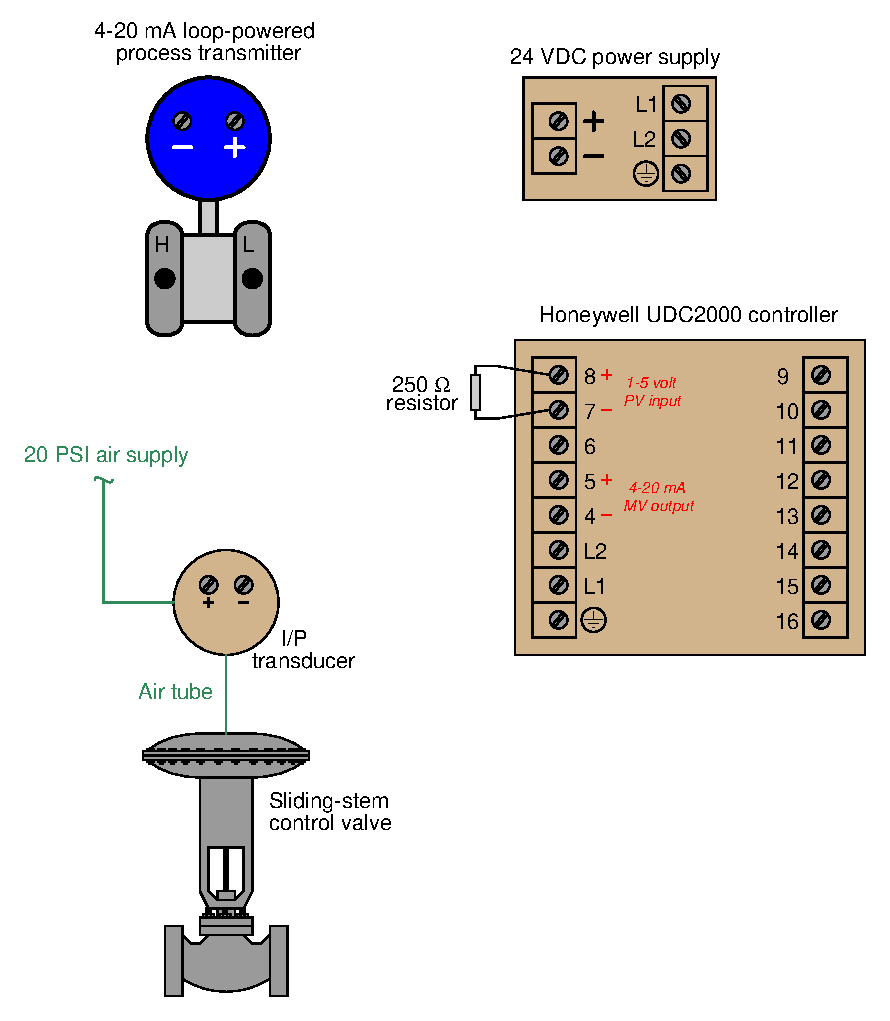
\includegraphics[width=15.5cm]{i00009x02.eps}$$


\vfil

Dette spørsmålet er typisk for dem i arbeidsarket ``Pictorial Circuit Diagrams'' som finnes i {\it Socratic Instrumentation} sin samling av øvingsark, bortsett fra at alle svar er gitt for disse spørsmålene.  Bruk gjerne dette øvingsarket som supplement til studiene dine av dette svært viktige temaet.

\underbar{file i00009}
\eject
%(END_QUESTION)





%(BEGIN_ANSWER)

Dette er et vurdert spørsmål -- ingen svar eller hint gis!

%(END_ANSWER)





%(BEGIN_NOTES)

$$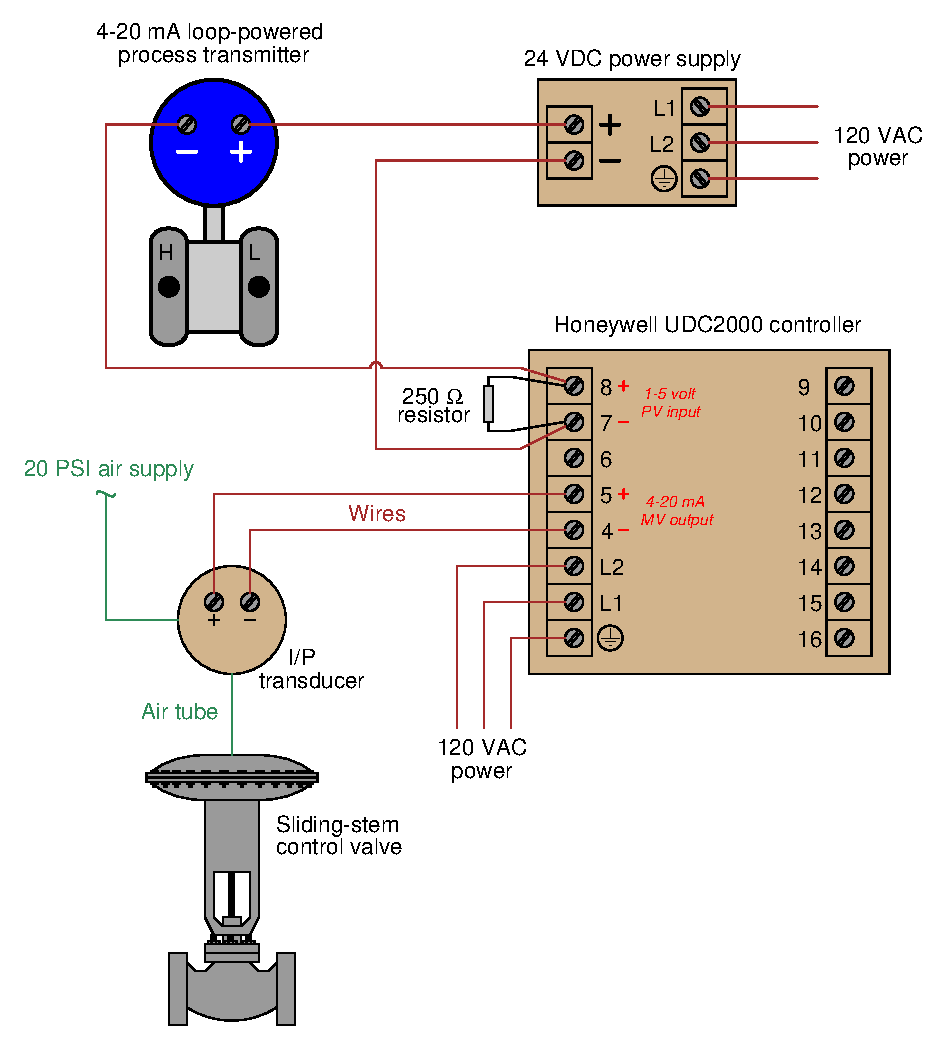
\includegraphics[width=15.5cm]{i00009x01.eps}$$

%INDEX% Pictorial circuit review (analog signal wiring to process controller)

%(END_NOTES)
